\chapter{Program organization and compilation script}
\label{sc:info}
\index{Programming organization and compilation}

\label{loc:contenu}

All the elements of the LMD model are in the {\bf LMDZ.GENERIC} directory
(and subdirectories).
As explained in Section~\ref{loc:contact1}, this directory
should be associated with
 environment variable {\bf LMDGCM}:\\
If using Csh:
\begin{verbatim}
setenv  LMDGCM /where/you/put/the/model/LMDZ.GENERIC
\end{verbatim}
If using Bash:
\begin{verbatim}
export  LMDGCM=/where/you/put/the/model/LMDZ.GENERIC
\end{verbatim}

\noindent Here is a brief description of the
{\bf LMDZ.GENERIC} directory contents:
\begin{verbatim}
  libf/  All the model FORTRAN Sources (.F or .F90)
         and  include files (.h) organised in sub-directories
        (physics (phystd), dynamics (dyn3d), filters (filtrez)...)

  deftank/   A collection of examples of parameter files required
                to run the GCM (run.def, callphys.def, ...)

  makegcm  Script that should be used to compile the GCM as well
            as related utilities (newstart, start2archive, testphys1d)

  create_make_gcm   Executable used to create the makefile.
                    This command is run automatically by
                    "makegcm" (see below).

\end{verbatim}


\section{Organization of the model source files}
\index{Organization of the model source files}

The model source files are stored in various sub directories
in directory {\bf libf}.
These sub-directories correspond to the different parts of the model:

\begin{description}
\item{\bf grid:} mainly made up of "dimensions.h" file,
which contains the parameters that define the model grid,
i.e. the number of points in longitude (IIM), latitude (JJM) and altitude
(LLM), as well as the number of tracers (NQMX).

\item{\bf dyn3d:} contains the dynamical subroutines.

\item{\bf bibio:} contains some generic subroutines not specifically
related to physics or dynamics but used by either or both.

\item{\bf phymars:} contains the physics routines.

\item{\bf filtrez:} contains the longitudinal filter sources applied in the
upper latitudes,
where the Courant-Friedrich-Levy stability criterion is violated.

\end{description}

\section{Programming}

The model is written in {\bf Fortran-77} and {\bf Fortran-90}.
\begin{itemize}
\item The program sources are written in {\bf ``file.F"}
or {\bf ``file.F90''} files.
The extension .F is the standard extension for fixed-form Fortran and
the extension .F90 is for free-form Fortran.
These files must be preprocessed (by a{\bf C preprocessor}
such as (cpp)) before compilation (this behaviour is, for most
compilers, implicitly obtained but using a capital F in the extention
of the file names).

\item Constants are placed in COMMON declarations,
located in the common ``include'' files {\bf "file.h"}

%\item [also module files now too...]
\item In general, variables are passed from subroutine to subroutine
as arguments (and never as COMMON blocks).

\item In some parts of the code, for ``historical'' reasons,
the following rule is sometimes used: in the subroutine,
the variables (ex: \verb+name+) passed as an argument by the calling program
are given the prefix \verb+p+ (ex: \verb+pname+)
 while the local variables are given the prefix \verb+z+ (ex: \verb+zname+).
As a result, several variables change their prefix (and thus their name)
when passing from a calling subroutine to a called subroutine. We're trying to eliminate this as the code is developed.
\end{itemize}

\section{Model organization}
Figure~\ref{fg:organi_phys} describes the main subroutines called by physiq.F. OBSOLETE - FOR MARS ONLY!!!
\index{Model organization}
\begin{figure}
\begin{flushleft}
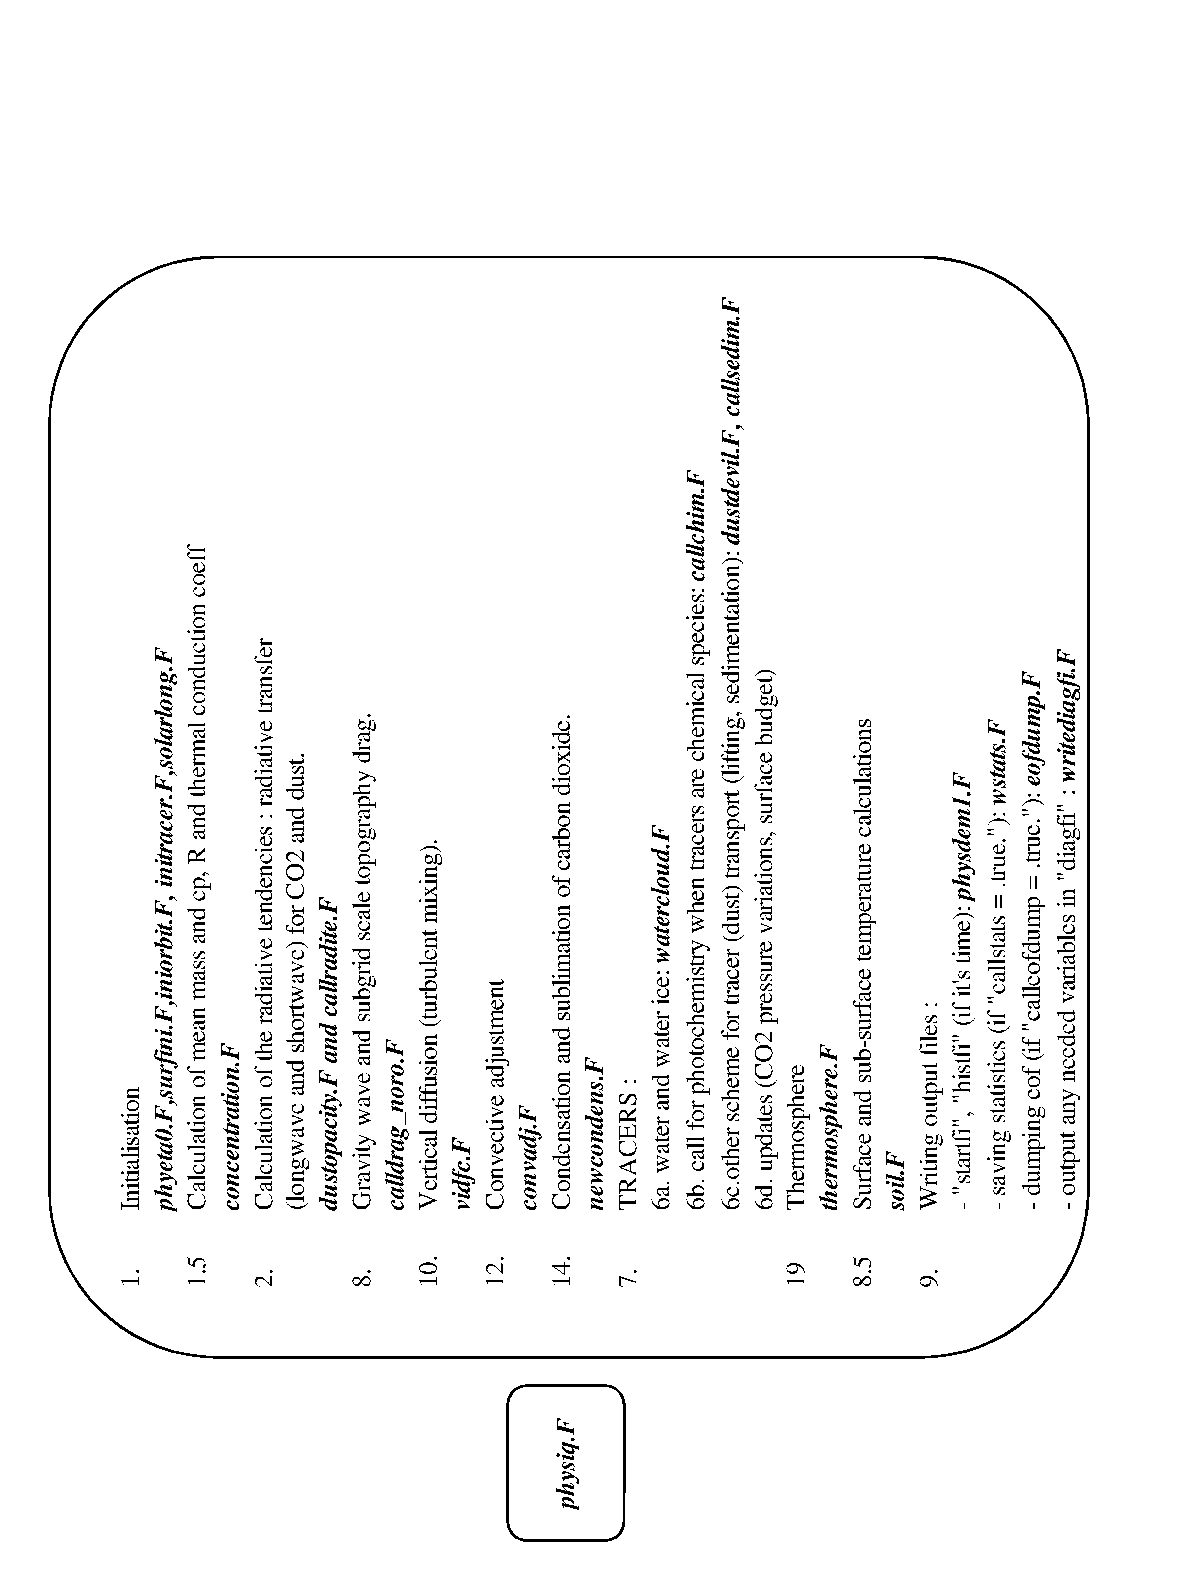
\includegraphics[scale=0.70,angle=-90]{Fig/physique.eps}
\caption{Organigram of subroutine function physiq.F90}
\label{fg:organi_phys}
\end{flushleft}
\end{figure}


%%%%%%%%%%%%%%%%%%%%%%%%%%%%%%%%%%%%%%%%%%%%%%%%%%
%  Compilation du modele
%%%%%%%%%%%%%%%%%%%%%%%%%%%%%%%%%%%%%%%%%%%%%%%%%%

\section{Compiling the model}
\index{Compiling the model}

\label{sc:compil1}
Technically, the model is compiled using the Unix utility {\tt make}.
The file {\tt makefile}, which describes the code dependencies
and requirements,
is created automatically by the script
\begin{verbatim}
create_make_gcm
\end{verbatim}
This utility script recreates the {\tt makefile} file when necessary,
for example, when a source file has been added or removed since the last
compilation.

{\bf None of this is visible to the user.
To compile the model just run the command}
\begin{verbatim}
makegcm
\end{verbatim}
with adequate options (e.g. {\tt makegcm -d 62x48x32 -p mars gcm}), as
discussed below and described in section~\ref{sc:run1}.


The {\tt makegcm} command compiles the model ({\bf gcm}) and related utilities
({\bf newstart}, {\bf start2archive}, {\bf testphys1d}).
A detailed description of how to use it and of the various parameters that
can be supplied
is given in the help manual below
(which will also be given by the \verb+makegcm -h+ command).\\
Note that before compiling the GCM with {\tt makegcm} you should have set
the environment variable {\bf LIBOGCM} to a path where intermediate
objects and libraries will be generated.\\
If using Csh:
\begin{verbatim}
setenv  LIBOGCM /where/you/want/objects/to/go/libo
\end{verbatim}
If using Bash:
\begin{verbatim}
export  LIBOGCM=/where/you/want/objects/to/go/libo
\end{verbatim}
\paragraph{Help manual for the makegcm script}
%%%%%%%%%%%%%%%%%%%%%%%%%%%%%%%%%%%%%%%%%%%%%%%%%%%%%%%
% makegcm.help:  lu dans makegcm
%%%%%%%%%%%%%%%%%%%%%%%%%%%%%%%%%%%%%%%%%%%%%%%%%%%%%%%
{\footnotesize
\begin{verbatim}
makegcm [Options] prog


The makegcm script:
-------------------

1. compiles a series of subroutines located in the $LMDGCM/libf
 sub-directories.
 The objects are then stored in the libraries in $LIBOGCM.

2. then, makegcm compiles program prog.f located by default in
$LMDGCM/libf/dyn3d and makes the link with the libraries.

Environment Variables '$LMDGCM' and '$LIBOGCM'
 must be set as environment variables or directly
 in the makegcm file.

The makegcm command is used to control the different versions of the model
 in parallel, compiled using the compilation options 
 and the various dimensions, without having to recompile the whole model.

The FORTRAN libraries are stored in directory $LIBOGCM.


OPTIONS:
--------

The following options can either be defined by default by editing the
makegcm "script", or in interactive mode:

-d imxjmxlm  where im, jm, and lm are the number of longitudes,
             latitudes and vertical layers respectively.

-t ntrac   Selects the number of tracers present in the model

             Options -d and -t overwrite file 
             $LMDGCM/libf/grid/dimensions.h
             which contains the 3 dimensions of the
             horizontal grid 
             im, jm, lm plus the number of tracers passively advected
             by the dynamics ntrac,
             in 4 PARAMETER FORTRAN format 
             with a new file:
             $LMDGCM/libf/grid/dimension/dimensions.im.jm.lm.tntrac
             If the file does not exist already
             it is created by the script
             $LMDGCM/libf/grid/dimension/makdim

-p PHYS    Selects the set of physical parameterizations
           you want to compile the model with.
           The model is then compiled using the physical
           parameterization sources in directory:
            $LMDGCM/libf/phyPHYS

-g grille  Selects the grid type.
           This option overwrites file
           $LMDGCM/libf/grid/fxyprim.h
           with file
           $LMDGCM/libf/grid/fxy_grille.h
           the grid can take the following values:
           1. reg - the regular grid
           2. sin - to obtain equidistant points in terms of sin(latitude)
           3. new - to zoom into a part of the globe

-O "compilation options" set of fortran compilation options to use

-include path
           Used if the subroutines contain #include files (ccp) that 
           are located in directories that are not referenced by default.

-adjnt     Compiles the adjoint model to the dynamical code.

-filtre  filter
           To select the longitudinal filter in the polar regions.
           "filter" corresponds to the name of a directory located in
           $LMDGCM/libf. The standard filter for the model is "filtrez"
           which can be used for a regular grid and for a  
           grid with longitudinal zoom.

-link "-Ldir1 -lfile1 -Ldir2 -lfile2 ..."
           Adds a link to FORTRAN libraries
           libfile1.a, libfile2.a ... 
           located in directories dir1, dir2 ...respectively
           If dirn is a directory with an automatic path 
           (/usr/lib ... for example) 
           there is no need to specify  -Ldirn.

\end{verbatim}
}

%%%%%%%%%%%%%%%%%%%%%%%%%%%%%%%%%%%%%%%%%%%%%%%%%%%%%%%
